\section{Revision for Homogeneous Electron Gas}
\label{HEG}

In this section, we describe how we adapt our SHCI algorithm to the homogeneous electron gas problem in the mid to high density region.
Appendix~\ref{app:heg} gives the Hamiltonian matrix elements of HEG.
HEG systems differ from other chemical systems that SHCI has been applied to in two ways: a large number of orbitals and plane wave basis sets.

\subsection{Large Basis Set}
In the mid to high density region, the correlation energy obtained from a finite basis set depends significantly on the size of the basis set.
Hence, in order to achieve high accuracy for the infinite basis set, we have to use a large number of orbitals, which is one to two orders of magnitude larger than what SHCI calculations used.

To reduce storage and improve speed when using a large basis set, we introduce a new way for representing the determinants.
First, the orbitals are sorted into descending order of importance.
Then, we use bit-packing for orbitals 1 to 128, and use a self-balancing binary search tree, called red-black tree~\cite{wiki:redblacktree}, to store the indices of the other occupied orbitals.
Fig.~\ref{fig:hybrid} illustrates this hybrid structure.
The red-black tree is a common data structure for storing a set of distinct objects, which in our case are the indices of the occupied orbitals. The worst case time complexity of both the insertion operation and the deletion operation on a red-black tree is $O(\log N)$.
\begin{figure}
  \begin{center}
  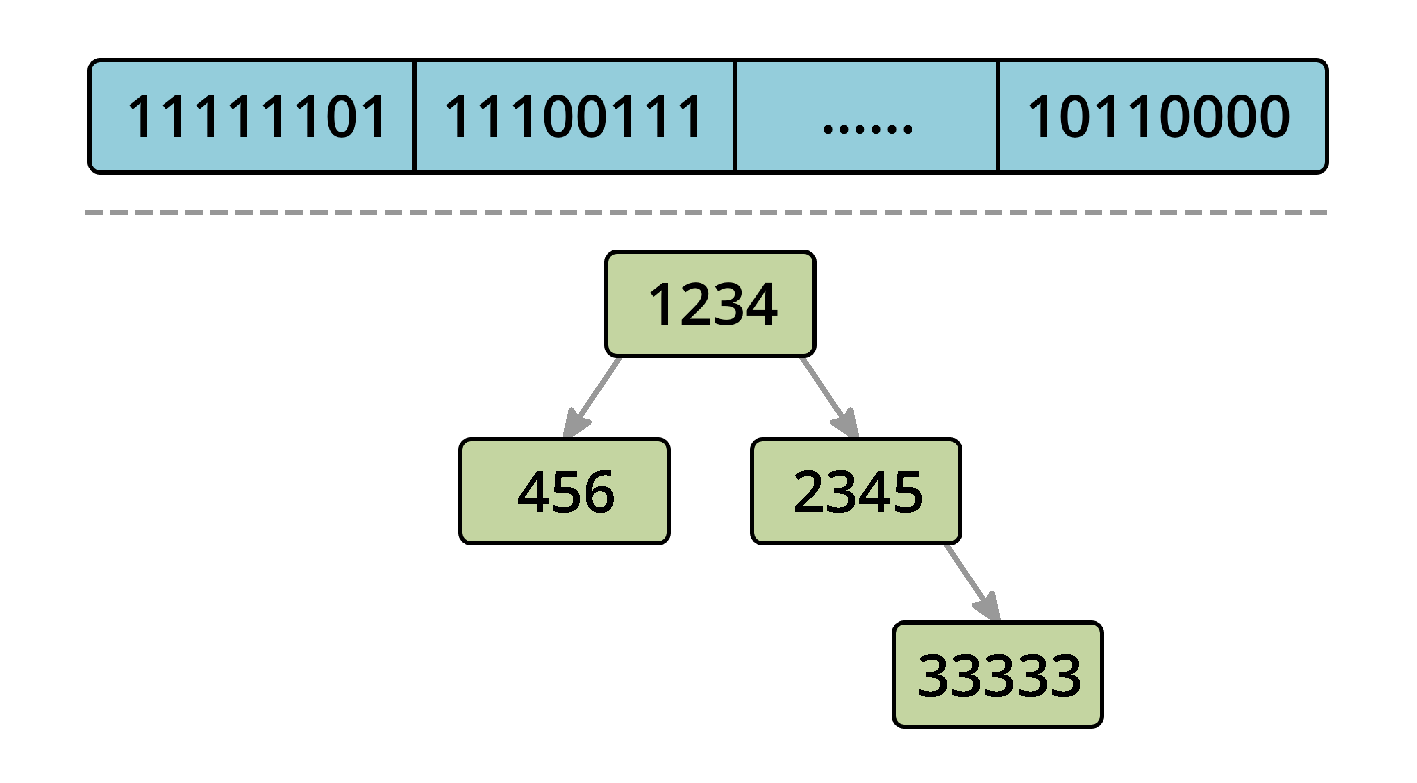
\includegraphics[width=0.9\linewidth]{figs/HybridDet.eps}
  \end{center}
  \vspace{-0.2cm}
  \caption{Hybrid Representation for Determinants.
  The occupancy of the most important 128 orbitals is represented with bit-packing.
  The indices of the other occupied orbitals are stored in a self-balancing binary search tree~\cite{wiki:redblacktree}.
  }
  \label{fig:hybrid}
\end{figure}

The usage of this hybrid structure gives us high performance and compact storage for both the small number of important orbitals and a large number of nonimportant orbitals.

\subsection{Orbital Momentum Conservation}
We solve HEG under a plane wave basis set and periodic boundary condition.
One property of this basis set is that each orbital have a specific momentum associated with it, and thus we can use momentum conservation to reduce the storage of the HCI double excitation helper lists.

First, we find all the possible differences between the momentum of two orbitals.
Let $M$ be the number of orbitals ($k$ points), then the number of distinct differences between them is also of order $O(M)$.
For an orbital $i$, we denote the momentum of that orbital to be $k_{i}$.
We use $p$ and $q$ to denote the pair of occupied orbitals during excitation, and $r$ and $s$ to denote the pair of unoccupied orbitals to which the electrons are excited.
Then we have $k_p + k_q = k_r + k_s$.
For HEG, as shown in Appendix~\ref{app:heg}, $k_p - k_q$ and $k_p - k_r$ uniquely determines the magnitude of the Hamiltonian matrix element associated with excitation $pq\to rs$.
Hence, for each possible momentum difference $k_{pq}$, we associate with it a list of $\langle k_{pr}, |H_{pqrs}|\rangle$ pairs in descending order of $|H_{pqrs}|$.
Fig.~\ref{fig:helper} illustrates the structure of these helper lists.
Finally, when using these helper lists to find important connected determinants to a given reference determinant, we perform the following for each pair of occupied orbitals $p$ and $q$: we go through the list associated with $k_{pq} = k_p - k_q$ to get $k_{pr}$ until the corresponding $|H_{pqrs}|$ falls below a given threshold.
Using $k_{pr}$ and momentum conservation, we can easily get $r$ and $s$, and thus the connected determinant which satisfies the SHCI criteria.
\begin{figure}
  \begin{center}
  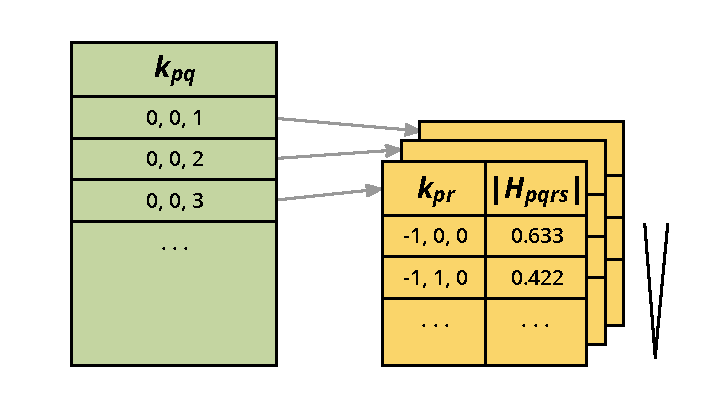
\includegraphics[width=0.9\linewidth]{figs/HelperList.eps}
  \end{center}
  \vspace{-0.2cm}
  \caption{SHCI Helper Lists for HEG.
  For each $k_{pq}$, we generate a list of $\langle k_{pr}, |H_{pqrs}|\rangle$ pairs and sort them into descending order of $|H_{pqrs}|$.
  When trying to find connected determinants from a given spawning determinant, we go through each occupied pair of orbitals $p$ and $q$, calculate their momentum difference $k_{pq}$, and go through the corresponding list until $|H_{pqrs}|$ falls below a certain threshold.
  For each entry that we go through in the list, we can obtain $r$ and $s$ by using $k_{pr}$ and momentum conservation.
  }
  \label{fig:helper}
\end{figure}

The storage complexity of these helper lists is $O(M^2)$, as opposed to $O(M^4)$ for chemistry systems.
The time complexity of finding determinants connected to a given determinant in descending order of importance is the same as in chemistry, which is $O(n_e^2 + n_D)$, where $n_e$ is the number of electrons and $n_D$ is the number of new determinants found.
